% !TeX spellcheck = nl_NL
%%%%%%%%%%%%%%%%%%%%%%%%%%%%%%%%%%%%%%%%%
% University Assignment Title Page 
% LaTeX Template
% Version 1.0 (27/12/12)
%
% This template has been downloaded from:
% http://www.LaTeXTemplates.com
%
% Original author:
% WikiBooks (http://en.wikibooks.org/wiki/LaTeX/Title_Creation)
%
% License:
% CC BY-NC-SA 3.0 (http://creativecommons.org/licenses/by-nc-sa/3.0/)
% 
% Instructions for using this template:
% This title page is capable of being compiled as is. This is not useful for 
% including it in another document. To do this, you have two options: 
%
% 1) Copy/paste everything between \begin{document} and \end{document} 
% starting at \begin{titlepage} and paste this into another LaTeX file where you 
% want your title page.
% OR
% 2) Remove everything outside the \begin{titlepage} and \end{titlepage} and 
% move this file to the same directory as the LaTeX file you wish to add it to. 
% Then add \input{./title_page_1.tex} to your LaTeX file where you want your
% title page.
%
%%%%%%%%%%%%%%%%%%%%%%%%%%%%%%%%%%%%%%%%%
\title{Paper Wetenschapsfilosofie: Technologie na de mens}
%----------------------------------------------------------------------------------------
%	PACKAGES AND OTHER DOCUMENT CONFIGURATIONS
%----------------------------------------------------------------------------------------

\documentclass[12pt]{article}
\usepackage[utf8x]{inputenc}
\usepackage[english]{babel}
\usepackage{amsmath}
\usepackage{graphicx}
\usepackage{float}
\usepackage[colorinlistoftodos]{todonotes}
\usepackage{hyperref}
\hypersetup{colorlinks = false, allbordercolors = {white}}

\begin{document}

\begin{titlepage}

\newcommand{\HRule}{\rule{\linewidth}{0.5mm}} % Defines a new command for the horizontal lines, change thickness here

\center % Center everything on the page
 
%----------------------------------------------------------------------------------------
%	HEADING SECTIONS
%----------------------------------------------------------------------------------------

\textsc{\LARGE Universiteit Hasselt}\\[1.5cm] % Name of your university/college
\textsc{\Large Wetenschapsfilosofie}\\[0.5cm] % Major heading such as course name

%----------------------------------------------------------------------------------------
%	TITLE SECTION
%----------------------------------------------------------------------------------------

\HRule \\[0.4cm]
{ \huge \bfseries Technologie na de mens}\\[0.4cm] % Title of your document
\HRule \\[0.5cm]
 
%----------------------------------------------------------------------------------------
%	AUTHOR SECTION
%----------------------------------------------------------------------------------------




% If you don't want a supervisor, uncomment the two lines below and remove the section above
\Large \emph{Door:}\\
Niels \textsc{Desair} (1436732)
\linebreak
Bram \textsc{Kelchtermans} (1437654) \\ % Your name

%----------------------------------------------------------------------------------------
%	DATE SECTION
%----------------------------------------------------------------------------------------

{\large 14 december 2016}\\[1cm] % Date, change the \today to a set date if you want to be precise

%----------------------------------------------------------------------------------------
%	LOGO SECTION
%----------------------------------------------------------------------------------------


\includegraphics{logo.png}\\[1cm] % Include a department/university logo - this will require the graphicx package
 
%----------------------------------------------------------------------------------------

\vfill % Fill the rest of the page with whitespace

\end{titlepage}

\tableofcontents
\newpage

\section{Introductie}
Wat zou er gebeuren met de technologie en de planeet als de mens ineens zou verdwijnen? Het klinkt als een vreemde vraag, maar is het dat wel? In een geologische oogwenk heeft de mens enorm veel verwezenlijkt, binnen een paar duizend jaar zijn steden, maatschappijen, monumenten en wetenschap gegroeid tot waar we nu zijn.\newline\newline
Na zo'n lange tijd op deze planeet heeft de aarde zich aangepast aan de mensen. Kan de natuur nog verder zonder ons? Wat laten we achter, zullen de sporen van ons bestaan ooit echt weg zijn? Wat gebeurt er met onze elektriciteit, monumenten, technologie, radioactiviteit en afval? Wat met de fauna en flora, en als er terug intelligent leven komt, zullen ze merken dat wij bestaan hebben of zullen alle sporen van ons bestaan weggevaagd zijn? Dit zijn allemaal vragen die wij hier zullen trachten te beantwoorden.
\section{Elektriciteit}
Vanuit de ruimte is het meest duidelijke bewijs dat de mens hier is de verlichting van onze straten en steden. (zie figuur \ref{fig:space}) \cite{lightsSpace} Maar hoe lang blijft dit zo? Hoe lang zullen de lichten blijven branden en welke regio's blijven het langste verlicht?\newpage
\begin{figure}
	\centering
	\includegraphics[width=0.9\textwidth]{space.jpg}
	\caption{De verlichting zichtbaar vanuit de ruimte}
	\label{fig:space}
\end{figure}
De meeste elektrische apparaten en lichten zullen binnen enkele uren al uitvallen. Dit omdat fossiele brandstoffen en kerncentrales het grootste aandeel innemen van onze energieproductie. \cite{energySources} Eerst zullen alle kerncentrales uitvallen vanwege veiligheidsprocedures, in iedere centrale moet namelijk om de paar uren op een fysieke knop gedrukt worden door een mens om de centrale aan de praat te houden \cite{standaard}, wat natuurlijk niet meer zal gebeuren. Ook zullen de fossiele brandstofcentrales (steenkool, aardgas) snel uitvallen aangezien de mens geen nieuwe brandstof meer zal bijvullen. \cite{standaard} Dit zorgt er dus voor dat enkel windmolens, zonnepanelen en waterdrukcentrales werkend blijven.\newline\newline
Echter zal het slechts een kwestie van weken of maanden zijn voor de windmolens en zonnepanelen het zullen begeven. De windmolens zullen blokkeren en er zal een laag stof op de zonnepanelen komen, waardoor deze niet voldoende energie meer produceren. \cite{standaard} Waterdrukcentrales zoals het wereldberoemde Hoover Dam zullen de enige nog werkende vorm van elektriciteit zijn en nog jaren doorgaan. Hierdoor zal de westkust van de Verenigde Staten de laatste verlichte plek op aarde zijn. \cite{hoover}
\section{Dieren}
Veel dieren zijn afhankelijk geworden van de mens. Dus wat gebeurt er met deze dieren als de mens uitsterft? We bekijken dit op verschillende vlakken. Zo zullen we het hebben over huisdieren zoals wij ze kennen, maar ook de wilde dieren in de natuur of in gevangenschap (zoals in een dierentuin ). Deze dieren zijn allemaal (on)rechtstreeks afhankelijk van de mens.  \cite{ASAPScience,LAPOutbreak}
\subsection{Huisdieren}
Logisch gezien zijn huisdieren het meest afhankelijk van de mens. Deze dieren zijn namelijk geconditioneerd waardoor veel van hun instincten naar de achtergrond verdwenen zijn. Wanneer de mens plots van de planeet zou verdwijnen zitten veel van deze huisdieren nog opgesloten in huis en/of een kooi. Deze dieren zullen geen eten of drinken meer krijgen en gaan zo beroep doen op hun instincten. Er zijn over het algemeen twee mogelijke scenario's die zich kunnen afspelen.
\newline\newline
Het eerste mogelijke scenario is dat de dieren geen mogelijkheid hebben om uit te breken. Denk zo maar aan vogels die in een afgesloten kooi zitten, vissen die logisch gezien niet kunnen ontsnappen uit het aquarium, honden die geen uitweg zien naar buiten etc. Zonder de hulp van de mens zijn deze dieren gedoemd om te sterven aan uitdroging of ondervoeding.
\newline\newline
De tweede optie is dat de dieren wel een optie tot ontsnappen hebben. Zoals al eerder vermeld heeft de mens het dierlijk instinct van huisdieren naar de achtergrond geduwd. Daarom zijn het ook huisdieren en geen wilde dieren. Als deze dieren dan toch in de natuur komen moeten deze toch beroep kunnen doen op hun instinct. Dit zal bij elk dier verschillend verlopen. Wat we wel kunnen zeggen is dat kleine dieren, zoals kleine hondjes en katten, niet lang zullen overleven in de wildernis. Dit doordat grotere dieren, zoals grotere honden en roofdieren, zullen gaan jagen op deze kleinere dieren. Verder in dit hoofdstuk wordt er ook gesproken over het feit dat veel wilde dieren (en dus ook roofdieren) dichter naar de (eerder) bewoonde wereld zullen komen. Dit zorgt er voor dat kleine dieren een geringe kans op overleven hebben. 
\newline
\begin{figure}
  \centering
    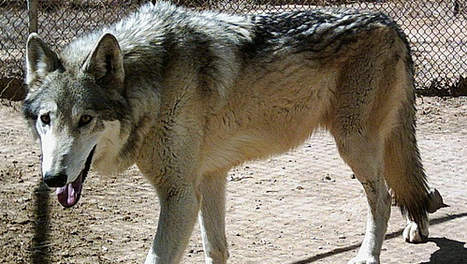
\includegraphics[width=0.9\textwidth]{WolfHond.jpg}
  \caption{Kruising tussen een wolf en een hond \cite{redactieHLN}}
  \label{fig:wolfhond}
\end{figure}
Als men denkt aan huisdieren denkt men natuurlijk aan de hond, de beste vriend van de mens. Daarom dat we even dieper in gaan op het leven van een hond na het verdwijnen van de mens. Zoals al eerder vermeld zullen kleine honden geen grote slaagkans op overleven hebben. Grote honden daarentegen hebben nog een groot deel van hun jachtinstinct kunnen behouden. Dit doordat deze honden vaak in de jacht gebruikt worden of dat er vaak spelenderwijs beroep wordt gedaan op hun instinct. Deze honden hebben dan weer een grotere kans op overleven, zij zullen immers sneller gaan jagen om zo voedsel te vinden. Aangezien alle huisdieren in het begin nog in de stad zullen zijn, zullen de kleinere huisdieren er eerst aan moeten geloven. Wat ook wel interessant is, is het feit dat wilde dieren zoals wolven dichter naar de dorpen zullen komen. Dit brengt met zich mee dat honden en wolven gaan kruisen en zo gaan zorgen voor nakomelingen. Dit zal er voor zorgen dat de hond na verloop van tijd zal verdwijnen en 'terug' zal evolueren naar de wolf, op figuur \ref{fig:wolfhond} is een foto te zien van een kruising tussen een wolf en een hond.
\subsection{Boerderijdieren}
De dieren op de boerderij leven altijd in gevangenschap, maar aangezien de elektriciteit na verloop van tijd zal uitvallen zullen veel van deze dieren uitbreken. Veel dieren zullen hierdoor prooi worden voor roofdieren of uitgebroken huisdieren. Andere dieren zullen vluchten en terug naar hun wilde vorm terugkeren. We denken hier dan bijvoorbeeld aan paarden, die ook een wilde vorm in de natuur hebben.
\subsection{Dierentuin}
De dieren in de dierentuin zullen ook gevangen zitten in kooien en geen voedsel meer kunnen krijgen. Veel van deze dieren zullen eventueel kunnen uitbreken uit hun gevangenschap.Doordat de dieren niet getemd of geconditioneerd zijn en dus nog wilde dieren zijn, zullen deze gemakkelijker kunnen overleven in de wildernis. Dit kan er voor zorgen dat er nijlpaarden door de rivieren in Zuid-Amerika zullen zwemmen of kamelen door de landschappen van Australi\"{e} zullen dwalen \cite{ASAPScience}.
\subsection{Wilde dieren}
Een andere groep dieren die we graag zouden bespreken zijn de wilde dieren. Deze dieren zijn op het eerste gezicht niet zo verwant met de mens maar niets is minder waar.
\newline
Zo zijn er dieren die schuw zijn van de mens en zich teruggetrokken hebben. Deze dieren zullen dichter tot de dorpen en steden komen doordat er geen mensen meer zijn waar ze bang voor moeten zijn. Hierdoor zullen er meer dieren in de dorpen rondlopen. Meer dieren betekent ook meer prooi, waardoor ook roofdieren zich zullen manifesteren in de steden.
\newline
De mens heeft er ook voor gezorgd dat veel dieren met uitsterven bedreigd zijn of al uitgestorven zijn. De dieren die momenteel met uitsterven bedreigd zijn zullen zich herstellen naar de normale proporties. Er is namelijk geen mens meer die leefruimte wegneemt of op ze jaagt. Zo zullen walvissen meer zeeruimte hebben en zich vermenigvuldigen naar de maximale capaciteit van onze oceanen \cite{LAPOutbreak}.

\newpage
\section{Constructies}
De mens heeft tal van constructies gebouwd tijdens zijn bestaan op de aarde. Denk zo aan de piramides in Egypte of het huis waar je nu in woont. Wat we zeker niet mogen vergeten zijn de ruimtetuigen die momenteel nog in een baan rond de aarde zitten. Maar wat gebeurt er met deze constructies nadat de mens verdwenen is? Er is namelijk niemand die de constructies zal repareren of renoveren. In dit hoofdstuk gaan we dieper in op de toekomst van de constructies die door menselijke handen zijn gemaakt.
\newline
\newline
Amper twee dagen na het verdwijnen van de mens zullen alle ondergrondse metrostations volgelopen zijn met water. Zonder de mens wordt namelijk het grondwater niet meer weggepompt. Een jaar hierna zullen alle ruimtetuigen neerstorten op de aarde doordat deze niet meer onder controle worden gehouden door mensen en dus hun baan verliezen. \cite{LAPOutbreak}
\newline
Na amper vijfentwintig jaar zal drie kwart van de bebouwde aarde terug begroeid zijn met vegetatie die daar behoort. Zo zullen onze steden veranderen in weilanden en bossen, terwijl steden zoals Las Vegas en Dubai zullen veranderen in woestijnen. De natuur neemt terug wat van hem is. \cite{ASAPScience, LAPOutbreak}
\newline
Onze huizen daarentegen zullen het langer volhouden, toch is dit een opvallend korte periode. Het zal namelijk vijftig tot honderd jaar duren voordat al onze huizen ingestort zullen zijn. We gaan er dan wel van uit dat er geen branden zijn ontstaan. Dit komt echter vaker voor zonder het toezicht van de mens. Wanneer namelijk \"{e}\"{e}n huis vuur vat, zal er niemand zijn om de vlammen onder controle te krijgen en het vuur zal zich dus onherroepelijk verspreiden naar de omliggende constructies of natuur. Ook termieten zullen er voor zorgen dat vele huizen instorten. \cite{ASAPScience,LAPOutbreak}
\newline
\begin{figure}
	\centering
	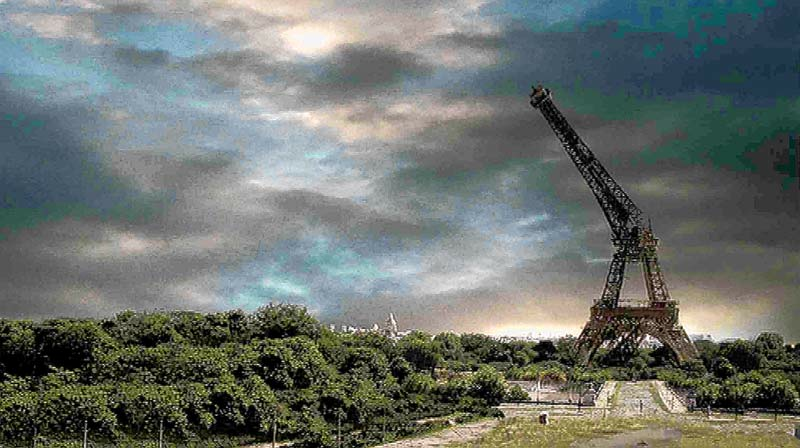
\includegraphics[width=0.9\textwidth]{EiffelToren.png}
	\caption{Instorten van de Eiffeltoren \cite{LAPOutbreak}}
	\label{fig:eiffel}
\end{figure}
\newline
Na ongeveer 300 jaar zullen de ijzeren constructies van de mens er ook aan moeten geloven. Zo zullen vele bruggen en ook de Eiffeltoren (zoals te zien in figuur \ref{fig:eiffel}) er aan moeten geloven. Dit doordat het ijzer zal roesten. Corrosie zorgt er ook voor dat het ijzer uitzet, dit tot drie maal zo groot. Dit zal er voor zorgen dat grote gebouwen, die veel ijzerwerk vereisen, zullen instorten. Na deze periode zal ook zo goed als elke dam ter wereld overstroomd of vernietigd zijn. Dit zal er voor zorgen dat Amerika bijvoorbeeld terug zal veranderen naar een moerassig landschap. Wat er dan weer voor zorgt er dan weer voor dat vele dieren kunnen terugkeren naar hun oorspronkelijke woonplaats.
\newline
Na een ongeveer tienduizend jaar zullen er nog maar enkele overblijfselen van onze gebouwen te zien zijn, we hebben het dan bijvoorbeeld over de piramides of de Chinese Muur. \cite{LAPOutbreak}

\newpage
\section{Afval}
Er is geen discussie mogelijk, de mens heeft veel afval, veel meer dan we waar we mee omkunnen. \cite{afval} Veel van dit afval zal simpelweg verbrandt worden, samen met de steden waar het opgeslagen ligt door onder andere de bliksem. Ook zal al het natuurlijk afbreekbaar afval verwijnen. Echter is er enorm veel onbrandbaar en onafbreekbaar afval \cite{ASAPScience}, wat gebeurt daarmee?\newline\newline
\begin{figure}
	\centering
	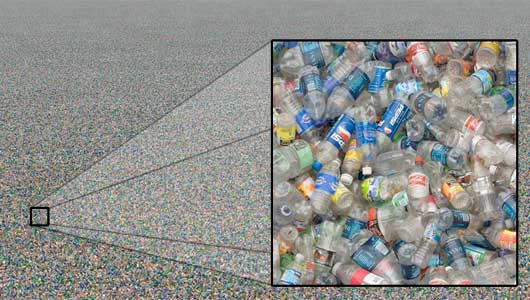
\includegraphics[width=0.9\textwidth]{plastic.jpg}
	\caption{Ophopen van plastic in de oceaan}
	\label{fig:plastic}
\end{figure}
Binnen honderd jaar zullen de meeste munstukken wegroesten door de regen en rivieren \cite{WorldWithoutUs} en de satellieten zullen uit de baan van de aarde vallen en op onze planeet landen. Roest en erosie zullen enorme schade doen aan al onze technologie, waar binnen enkele duizenden jaren niets meer van over zal blijven. \cite{standaard} Al het plastiek en ander onafbreekbaar afval zal zich verzamelen in natuurlijke sedimenten in het water (figuur \ref{fig:plastic}) en hier zeer lang blijven.\newpage Pas na ongeveer 30 miljoen jaar zal dit afval verdwenen zijn, opgeslokt en verteerd door de oceaan, echter zullen er nog 70 miljoen jaar langer sporen van te vinden zijn. Pas na 100 miljoen jaar zullen alle sporen van ons afval dus verteerd zijn.\cite{ASAPScience} \newline\newline
Maar het is de restanten en radioactiviteit van gesmolten atoombommen die het langste zullen blijven: het zal naar schatting 250 miljoen jaar duren voor dit volledig weg is. \cite{WorldWithoutUs}

\section{Radioactiviteit en andere stralingen}
Door de jaren heen heeft de mens veel ge\"{e}xperimenteerd met stralingen. Denk zo maar aan radio golven of mobiele stralingen om onze mobiele telefoons te voorzien van bereik. Een andere straling die we hier bespreken is de radioactieve straling. Deze stralingen zullen een grote inpakt hebben op de wereld zonder het toezicht van de mens.
\subsection{Radioactieve stralingen}
Na amper 7 dagen zal alle koelvloeistof voor kerncentrales opgebruikt zijn. Dit zorgt voor tal van explosies die veel erger zullen zijn dan de explosies in Fukushima of Chernobyl. Hierdoor zullen veel dieren sterven aan de gevolgen van kanker, dat veroorzaakt zal zijn door deze stralingen. Mutaties zullen ook veel vaker voorkomen bij de dieren die zich gevestigd hebben in de buurt van deze kerncentrales. Dit was namelijk ook het geval bij de kernrampen van Chernobyl en Fukushima, zoals te zien is in figuur \ref{fig:mutatielam}. De aarde zal hier echter vrij snel en vlot van herstellen.\cite{LAPOutbreak} 
\begin{figure}[h]
	\centering
	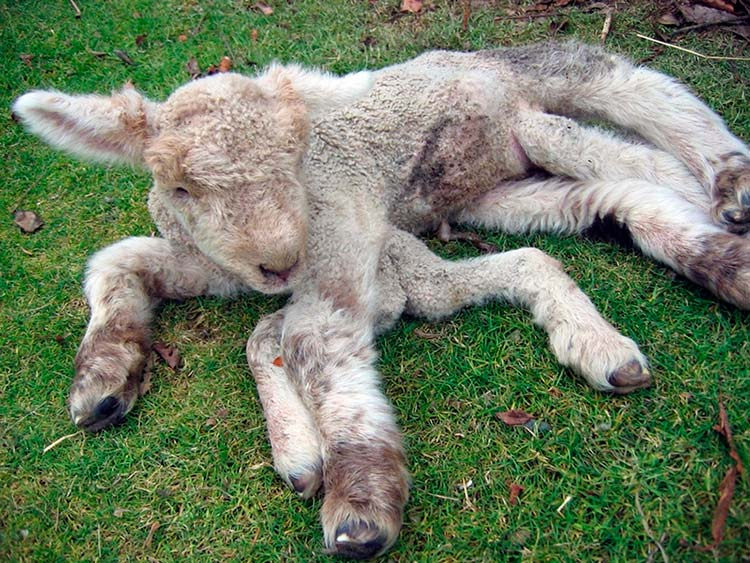
\includegraphics[width=0.8\textwidth]{ChernobylLam.jpg}
	\caption{Gemuteerd lam na de ramp in Chernobyl \cite{ChernobylMutations}}
	\label{fig:mutatielam}
\end{figure}
\newline\newline
Doordat de waarschuwingslichten van kernreactoren niet meer werken en de hoogspanningskabels verkillen, zullen er jaarlijks miljoenen vogels sterven aan de gevolgen van stralingen. Radioactieve straling zorgt namelijk voor warmte, wat vogels aantrekt.
\newline\newline
Een andere gevaarlijke stof waar de aarde mee te kampen gaat hebben is Plutonium. Deze stof heeft de mens gebruikt in bommen. Deze bommen zullen echter hun metalen mantel volledig verloren hebben na 250 000 jaar. Dit zorgt er dus voor dat de Plutonium en zijn straling vrijkomen in de natuur. De straling die van Plutonium komt kan bij inademing longkanker veroorzaken, dit kan gepaard gaan met andere stralingsziektes.\cite{WorldWithoutUs}
\newline\newline
Hoewel radioactieve straling een desastreuze werking zal hebben op het leven op aarde, zal de aarde er snel van herstellen. 
\subsection{Andere stralingen}
Stralingen is zeker geen onbekend begrip meer in deze tijd van moderne technologie. Ieder mens krijgt er dagelijks mee te maken. Denk zo maar aan draadloos internet, de auto radio, de mobiele telefoon etc. Al deze stralingen zijn door de mens gecre\"{e}erd en naar de buitenwereld gestuurd. 
\newline\newline
Als de mens echter plots verdwijnt van de aardbol zullen deze stralingen blijven bestaan, sterker nog dit zal het overblijfsel van de mens zijn dat het langste te vinden zal zijn op onze planeet. Maar niet enkel op onze planeet, onze radiogolven gaan verder. Zelfs na het vergaan van de aarde (geschat op ongeveer 5 biljoen jaar van nu \cite{WorldWithoutUs}) zouden onze radiogolven nog aanwezig zijn in het universum.
\section{Herstellen van natuur}
De mens is de grootste vervuiler van de aarde, dus wat zal de natuur doen als deze verdwijnt? Wetenschappers gebruiken vaak de zin: "De natuur neemt wat van hem is." We bekijken in dit hoofdstuk of dit ook daadwerkelijk het geval is.
\newline
\newline
Zonder de mens zal de lucht veel zuiverder worden. Het bekende fenomeen van smog (zie figuur \ref{fig:smog}) zal opgelost zijn. Het duurt echter ongeveer honderdduizend jaar voordat het \texorpdfstring{CO\textsubscript{2}}{2} gehalte teruggebracht is naar de normale proporties. 
\begin{figure}[h]
	\centering
	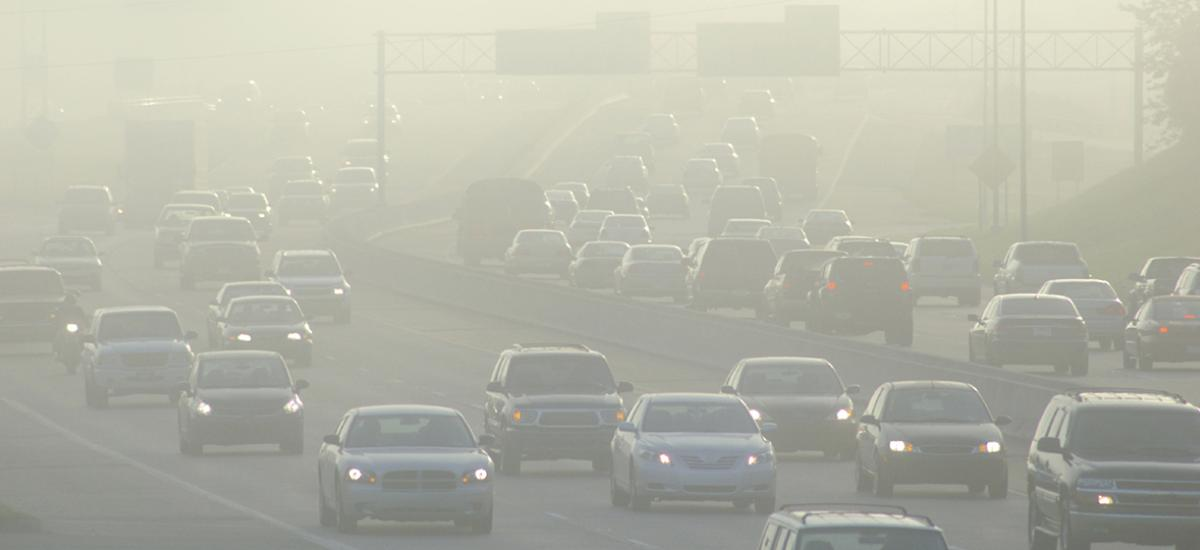
\includegraphics[width=0.8\textwidth]{LuchtVervuiling.jpg}
	\caption{Luchtvervuiling als gevolg van \texorpdfstring{CO\textsubscript{2}}{2} uitstoot \cite{Pollution}}
	\label{fig:smog}
\end{figure}
\newline\newline
Zoals al eerder vermeld zal de dierenpopulatie ook baat hebben bij het verdwijnen van de mens. Niet uitgestorven dieren zullen zich herstellen naar de maximale capaciteit die de aarde aan kan. Dit is zelfs het geval voor bedreigde diersoorten zoals walvissen, ijsberen etc.
\newline\newline
Na ongeveer tienduizend jaar zijn er enkel nog overblijfselen over van onze gebouwen. De piramides in Egypte zullen zelfs nog zo goed als volledig overeind staan. Andere monumenten, zoals Mt. Rushmore zullen nog een paar honderdduizend jaar overleven!
\newline\newline
Vijfendertigduizend jaar na het verdwijnen van de mens zal de loodvervuiling volledig verdwenen zijn. We spreken dan over de vervuiling die veroorzaakt is door het Industri\"{e}le tijdberk van ons bestaan.
\newline\newline
Iedere wetenschapper weet dat de mens een grote vervuiler is. Niet alleen de \texorpdfstring{CO\textsubscript{2}}{2} uitstoot van de mens, maar ook het afval dat we achterlaten zal een grote herstelperiode vragen. Ons afval is na vijftig miljoen jaar het enige overblijvende spoor van ons bestaan. Nog eens vijftig miljoen jaar verder (dus pas na honderd miljoen jaar!) zullen ook deze sporen verdwenen zijn en zal dus nergens uit blijken dat we ooit bestaan hebben.
\newline\newline
We springen nu verder in de tijd, we zijn nu vier en een half biljoen jaar verder na het verdwijnen van de mens. Na deze periode zal de aarde zeer sterk opgewarmd zijn doordat de zon groter en groter wordt. Veel leven verdwijnt door de toenemende hitte. Nog een half biljoen jaar later zal de aarde volledig opgebrand zijn. Toch is er dan nog een klein teken van onze civilisatie namelijk onze radiogolven die door de ruimte zullen blijven dwalen.
\newline
\newline
We kunnen dus zeggen dat de aarde zich volledig zal herstellen van ons bestaan. Het is echter wel een zeer lange en moeilijke revalidatie periode voor onze aardbol. Bedenk goed dat wij niet zonder de aarde kunnen, maar de aarde wel zonder ons!
\newpage
\section{Nieuw intelligent leven?}
Hoewel de kans zeer klein is dat er weer een wezen als de mens op de aarde zal lopen zeer klein is, is ze niet onbestaand. Als intelligente apen overleven, zou dit binnen 2,3 miljoen jaar al mogelijk kunnen zijn, aangezien dit de geschatte tijd is dat de mens nodig had om deze evolutie te maken. \cite{monkey} De vraag is dan natuurlijk, hoe lang zal dit nieuwe wezen nodig hebben om wetenschappelijk ver genoeg te staan om het bestaan van ons nog te merken?\newline\newline Het antwoord hierop is waarschijnlijk "te lang". Onze laatste overblijfselen van plastic in de oceanen zouden de laatste merkbare bewijzen van ons bestaan zijn, en de kans is dus zeer groot dat het nieuwe wezen zal denken dat zij de eerste intelligente beschaving op aarde zullen zijn. De natuur zal in zulke mate hersteld zijn van onze ingrepen dat het was alsof we er nooit waren. \cite{standaard} \newline\newline
Maar zelfs als ze van ons bestaan zouden afweten, is de vraag nog maar of we trots mogen zijn op wat we achterlaten voor hen. Afval, radioactiviteit en vernietiging, waren wij wel een goed voorbeeld, of zijn wij op het slechte pad? Dit zijn vragen die wij graag aan de lezer overlaten.\newpage

\section{Conclusie}
Binnen enkele jaren zal er geen elektriciteit meer zijn op aarde, onze technologische appareten zullen allemaal verdwenen zijn na honderden tot duizenden jaren. Hiermee is de technologie een van de eerste zaken die zal verdwijnen van onze planeet.\newline\newline
De fauna en flora zullen zich na een enorme klap herstellen, overlevende diersoorten zullen terugkeren naar de populaties van voor onze tussenkomst en ze zullen allemaal terug naar hun wilde vormen terugkeren. Ook zullen onze steden en monumenten na duizenden jaren allemaal verdwenen zijn.\newline\newline
Maar het blijft ons afval en onze vervuiling die het langste meegaat. De planeet zal zich perfect herstellen, maar dit zal een zeer, zeer lang proces zijn. Pas na ongeveer 100 miljoen jaar zal al ons afval verdwenen zijn. \newline\newline
De natuur zal dus herstellen en zal er beter aan toe zijn dan in de tijd dat de mensen er op rondliepen. Het moraal van het  verhaal? Wij hebben de natuur nodig, maar de natuur ons niet. Draag zorg voor haar, voor het te laat is.

\begin{thebibliography}{9}
\bibitem{lightsSpace}
	Deborah Byrd,
	\emph{How Earth looks from outer space},
	\url{http://earthsky.org/astronomy-essentials/in-space-how-far-away-can-you-see-earth}
	\bibitem{energySources}
	TSP Data,
	\emph{Breakdown of Electricity Generation by Energy Source},
	\url{http://www.tsp-data-portal.org/Breakdown-of-Electricity-Generation-by-Energy-Source}
		\bibitem{standaard}
		De Standaard,
		\emph{Dit gebeurt er met onze aarde als mensen uitsterven},
		\url{http://www.standaard.be/cnt/dmf20160601_02317919}
		\bibitem{hoover}
		U.S. Bureau of Reclamation,
		\emph{Hoover Dam facts},
		\url{https://www.usbr.gov/lc/hooverdam/faqs/powerfaq.html}
				\bibitem{afval}
				Derek Thompson,
				\emph{2.6 Trillion Pounds of Garbage: Where Does the World's Trash go?},
				\url{http://www.theatlantic.com/business/archive/2012/06/26-trillion-pounds-of-garbage-where-does-the-worlds-trash-go/258234/}
\bibitem{redactieHLN}
  Redactie HLN,
  \emph{Vergeet uw trouwe hond, haal een halve wolf in huis},
  Het Laatste Nieuws,
  2009.
 \bibitem{ASAPScience}
  Asap Science,
  \emph{What if humans disappeared?},
  \url{https://www.youtube.com/watch?v=guh7i7tHeZk},
  2015
 \bibitem{LAPOutbreak}
	Flight 33 Productions,
    \emph{Life After People},
    History,
    2008
\bibitem{WorldWithoutUs}
	Alan Weisman,
	\emph{The World Without Us},
	2007
\bibitem{ChernobylMutations}
	Chernobyl Guide,
	\emph{Chernobyl Mutations In Humans And Animals},
	\url{https://chernobylguide.com/chernobyl_mutations/}
\bibitem{Pollution}
	Union of Concerned Scientists,
	\emph{Vehicles, Air Pollution and Human Health},
	\url{http://www.ucsusa.org/clean-vehicles/vehicles-air-pollution-and-human-health#.WEwjqObhCUk}
	\bibitem{monkey}
	Friedemann Schrenk,
	\emph{The Earliest Putative Homo Fossils},
2007
	
\end{thebibliography}


\end{document}